  \parindent0pt
  \null
  \colorlet{mintgreen}{green!50!black!50}

  \thispagestyle{empty}
  \vskip3cm
  \vfill
  \hfil
  \begin{tikzpicture}[overlay]
    \coordinate (front) at (0,0);
    \coordinate (horizon) at (0,.31\paperheight);
    \coordinate (bottom) at (0,-.6\paperheight);
    \coordinate (sky) at (0,.57\paperheight);
    \coordinate (left) at (-.51\paperwidth,0);
    \coordinate (right) at (.51\paperwidth,0);

    \shade [bottom color=blue!30!black!10,top color=blue!30!black!50]
      ([yshift=-5mm]horizon -|  left) rectangle (sky -| right);
    \shade [bottom color=black!70!green!25,top
    color=black!70!green!10]
      (front -| left) -- (horizon -| left)
      decorate [decoration=random steps] { -- (horizon -| right) }
      -- (front -| right) -- cycle;
    \shade [top color=black!70!green!25,bottom color=black!25]
      (front -| left) -- (horizon -| left)
      decorate [decoration=random steps] { -- (horizon -| right) }
      -- (front -| right) -- cycle;
    \shade [top color=black!70!green!25,bottom color=black!25]
      ([yshift=-5mm-1pt]front -| left) rectangle ([yshift=1pt]front -|
      right);
    \fill [black!25] (bottom -| left) rectangle ([yshift=-5mm]front -|
    right);

    \def\nodeshadowed[#1]#2;{\node[scale=2,above,#1]{#2};\node[scale=2,
        above,#1,yscale=-1,scope fading=south,opacity=0.4]{#2};}

    \nodeshadowed [at={(-5,5  )},yslant=0.05]
        {\Huge Fun \textcolor{orange}{\emph{k}}of};
    % \nodeshadowed [at={( 0,5.3)}] {\huge \textcolor{mintgreen}{\&}};
    \nodeshadowed [at={( 5,5  )},yslant=-0.05] {\Huge \textsc{Programming}};
    \nodeshadowed [at={( 0,2  )}] {Advanced Programming In OCaml};

    \foreach \i in {0.5,0.6,...,2}
      \fill [white,decoration=Koch snowflake,opacity=.9]
            [shift=(horizon),shift={(rand*11,rnd*7)},scale=\i]
            [double copy shadow={opacity=0.2,shadow xshift=0pt,shadow
              yshift=3*\i pt,fill=white,draw=none}]
        decorate {
          decorate {
            decorate {
              (0,0) -- ++(60:1) -- ++(-60:1) -- cycle
            }
          }
        };
  \end{tikzpicture}
  \vfill
  
% \clearpage
% \newcommand\nbvspace[1][1]{\vspace*{\stretch{#1}}}
% % allow some slack to avoid under/overfull boxes
% \newcommand\nbstretchyspace{\spaceskip0.5em plus 0.25em minus 0.25em}
% % To improve spacing on titlepages
% \newcommand{\nbtitlestretch}{\spaceskip0.6em}

% \pagestyle{empty}

% \begin{center}
% \bfseries
% \nbvspace[1]
% \Huge
% {\nbtitlestretch\huge
%  Fun Of Programming }
% % \newline
% \nbvspace[1] 
% \scriptsize \textit{the tao produced one \\
% one produced two\\
% two produced three\\
% three produced all things\\ }

% \small \textit{By}\\
% \large \textit{Hongbo Zhang}\\[0.5em]

% \nbvspace[1]
% 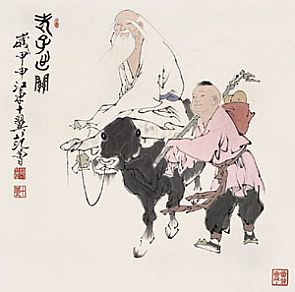
\includegraphics[width=4in]{./graphics/lao}

% \footnotesize University Of Pennsylvania

% \nbvspace[2]


% \nbvspace[3]
% \normalsize

% %% Hongbo Zhang\\
% \large
% Work In Progress
% \nbvspace[1]
% \end{center}

